\section{Our Approach}

A precise solution to the monitoring problem at hand would include considering all interleavings of the concurrent events in the given distributed signal.
The partial synchrony assumption helps reduce the number of such interleavings, however, the state-of-the-art leveraging this assumption relies on off-the-shelf SMT solvers and thus are not able to provide theoretical guarantees on running time and memory consumption~\cite{GangulyMB20,MomtazAB23}.
In order to design a dedicated monitoring algorithm with provable guarantees \borzoo{Do we do that?!}, we introduce the bounded variability assumption and a method to overapproximate the set of behaviors of the distributed signal.
We assume a central monitor that knows the values of $\varepsilon$ and $\delta$ as well as the initial values of the signals.

%TODO: add a short paragraph explaining each subsection

\subsection{Uncertainty Regions and Canonical Segmentations} \label{sec:segment}

Consider a signal $x : [0,d) \to \R$ with a single rising edge from value 2 to 3 at local time $t$.
The monitor observing this signal needs to take into account how the local clock of the agent producing $x$ relates with the global clock: due to clock skew, the rising edge of $x$ occurs in the range $(t - \varepsilon, t + \varepsilon)$ according to the global clock.
This range is called an \emph{uncertainty region} because in the interval $(t - \varepsilon, t + \varepsilon)$ the monitor cannot tell the value of $x$ precisely, but only that it changes from 2 to 3.
To systematically reason about uncertainty regions of signals, we use the notion of segmentation of temporal domains of signals.

Given a temporal domain $I = [0,d) \subset \R_{\geq 0}$, a \emph{segmentation} of $I$ is a partition of $I$ into finitely many intervals $I_1, \ldots, I_k$ of the form $I_j = [t_j, t_{j+1})$ such that $t_j < t_{j+1}$ for all $1 \leq j \leq k$.
By extension, a segmentation of a collection of signals with the same temporal domain $I$ is a segmentation of $I$. \borzoo{Are these consecutive intervals?}

Let $x : [0,d) \to \R$ be a signal and $E_x = \{(t_1, x(t_1)), \ldots, (t_m, x(t_m))\}$ be the set of edges of $x$, given in an increasing order of local clock values.
For $1 \leq i \leq m$, we let 
\begin{align*}
%	\theta_{\text{lo}}(x,t_i) &= \max\{0, \max_{j \in \{1, i\}} t_j - \varepsilon - (j-i)\delta\} \text{, and} \\
	\theta_{\text{lo}}(x,t_i) &= \max_{1 \leq j \leq i} t_j - \varepsilon + (i-j)\delta \text{, and} \\
	\theta_{\text{hi}}(x,t_i) &= \min_{i \leq j \leq m} t_j + \varepsilon - (j-i)\delta.
\end{align*}
Intuitively, $\theta_{\text{lo}}$ and $\theta_{\text{hi}}$ give us the lower and upper bounds on the value of the global clock for a given edge, i.e., the bounds on the uncertainty region of the edge.
We use these to describe a canonical segmentation of a distributed signal.

Let $(S,{\hb})$ be a distributed signal of $n$ signals.
For each signal $x_i$, let $F_i = \{\theta_{\text{lo}}(x_i, t_j) \st (t_j, x_i(t_j)) \in E_i\} \cup \{\theta_{\text{hi}}(x_i, t_j) \st (t_j, x_i(t_j)) \in E_i \}$ be the set of bounds on its uncertainty regions.
Let $d' = \max(d, \max (\bigcup_{i = 1}^{n} F_i))$, which corresponds to the duration of the distributed signal with respect to the global clock.\borzoo{why global clock?}
%
We define $F_S = \{0, d'\} \cup \bigcup_{i = 1}^{n} F_i$ and let $(a_j)_{1 \leq j \leq |F|}$ be an increasing sequence of clock values corresponding to the elements of $F$.
We define the \emph{canonical segmentation} of $(S,{\hb})$ as $G_S = \{I_1, \ldots, I_{|F| - 1}\}$ where $I_j = [a_j, a_{j+1})$ for all $1 \leq j < |F|$.

\begin{example} \label{ex:canonseg}
	Let $(S, {\hb})$ be a distributed signal with $S = (x_1, x_2)$ over the temporal domain $[0,8)$ such that $\pi(x_1) \neq \pi(x_2)$.\borzoo{$\pi$ is unnecessary.}
	Suppose $x_1(0) = 2$ and $x_2(0) = 3$, and let $\varepsilon = 2$ and $\delta = 3$.	
	Consider the case where $x_1$ has a rising edge $(3,5)$ and a falling edge $(5,3)$ while $x_2$ has a rising edge $(2,7)$ and a falling edge $(5,2)$.
	For $x_1$, taking into account only the clock skew would give us the uncertainty regions $(1,5)$ and $(3,7)$.\borzoo{We should this by a figure.}
	However, the computation of uncertainty regions take into account also the bounded variability.
	Intuitively, if the rising edge of $x_1$ occurs at global time 1, considering bounded variability, its falling edge occurs at the earliest at global time 4 instead of 3.
	Conversely, if the falling edge occurs at global time 7 then its rising edge occurs at the latest at global time 4 instead of 5.
	Then, we obtain $F_1 = \{1, 4, 7\}$.
	For $x_2$, the uncertainty regions are $(0,4)$ and $(3,7)$, which gives us $F_2 = \{0, 3, 4, 7\}$; and therefore, $F_S = \{0, 1, 3, 4, 7, 8\}$.
	This leads to the canonical segmentation $G_S = \{[0,1), [1,3) ,[3,4) ,[4,7) ,[7,8)\}$.		
\end{example}

\begin{figure} 
	\centering
	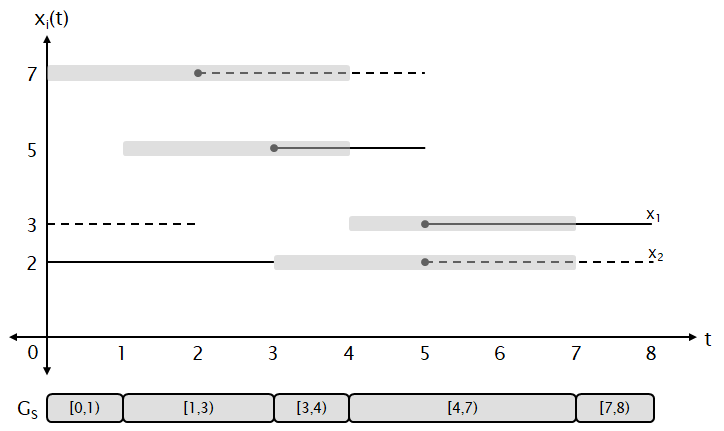
\includegraphics[scale=0.45]{canonseg.png}
	\caption{The values of $x_1$ (solid) and $x_2$ (dashed) over time. The edges are marked with black balls and their uncertainty regions are given as light gray boxes around the edges. The resulting canonical segmentation $G_S$ is shown below the graphical representation of the signals.\label{fig:canonseg}}
\end{figure}



\subsection{Value Expressions}
In uncertainty regions, although the monitor is not able to determine the exact value of a signal at a time point, it knows how the signal values change.
To capture this information, we use short sequences of possible signal values capturing how a signal behaves within a segment and several operations on them to propagate the information from real-valued signals to truth values of subformulas.

Let $\Sigma$ be a finite alphabet corresponding to a set of signal values.
A \emph{value expression} is a finite word in $\destutter(\Sigma^*)$.
Given value expressions $u_1$ and $u_2$, we define their \emph{asynchronous product} to encode their potential interleavings as follows:
\small
$$u_1 \otimes u_2 = \{ \destutter(v_1, v_2) \st v_i \in \stutter_k(u_i), \text{ where } k = |u_1| + |u_2| - 1\}$$  
\normalsize
Given $L_1, L_2 \subseteq \destutter(\Sigma^*)$, we write $L_1 \otimes L_2 = \{ u_1 \otimes u_2 \st u_i \in L_i\}$.

\borzoo{The definition if destutter is a unary function. The above is a binary function. Also, I think you should add $i \in \{1,2\}$}
For value expressions $u_1, u_2$ and a function $f : \Sigma^2 \to \R$, we refer to the set of value expressions that can be obtained by applying $f$ to their asynchronous product as follows: $f(u_1, u_2) = \destutter(\{(f(v_1[i], v_2[i]))_{1 \leq i \leq k} \st (v_1, v_2) \in u_1 \otimes u_2 \text{ and } k = |v_1| \})$.
Moreover, for $c \in \R$, we write $f(u_1, u_2) > c$ to denote the set $\destutter(\{(f(v_1[i], v_2[i]) > c)_{1 \leq i \leq k} \st (v_1, v_2) \in u_1 \otimes u_2 \text{ and } k = |v_1|\})$ where, for each $i$, the value of $f(v_1[i], v_2[i]) > c$ is 1 if the inequality holds, and it is 0 otherwise.
We naturally extend these definitions to functions of arbitrary (finite) arity.

\begin{example} \label{ex:valexpr}
	Recall the distributed signal $(S, {\hb})$ in \cref{ex:canonseg}.
	To encode the behavior of $x_1$ and $x_2$, let $\Sigma = \{2, 3, 5, 7\}$.
	One possible behavior of these signals is that the rising edge of $x_1$ and the falling edge of $x_2$ occur in the segment $[3,4)$.
	We represent this case by taking the value expression $u_1 = 2 \cdot 5$ for $x_1$ and $u_2 = 7 \cdot 2$ for $x_2$ in the segment $[3,4)$.
	To capture the potential interleavings of these edges, we compute the asynchronous product $u_1 \otimes u_2$ of these value expressions.
	Stuttering $u_1$ and $u_2$ up to length 3 and taking their product gives us
	$(2 \cdot 2 \cdot 5, 7 \cdot 7 \cdot 2)$,
	$(2 \cdot 2 \cdot 5, 7 \cdot 2 \cdot 2)$,
	$(2 \cdot 5 \cdot 5, 7 \cdot 7 \cdot 2)$, and
	$(2 \cdot 5 \cdot 5, 7 \cdot 2 \cdot 2)$.
	Observe that the first and the last pairs are equivalent after destuttering and they encode the case when the rising and falling edges occur exactly at the same time with respect to the global clock.
	On the other hand, the second (resp. third) pair encodes the case when the falling edge of $x_2$ occurs before (resp. after) the rising edge of $x_1$.
	
	Now, to compute the function $u_2 - u_1$ we apply the function letter by letter to the pairs in their asynchronous product.
	For example, applying it to $(2 \cdot 5, 7 \cdot 2)$ results in $(7 - 2) \cdot (2 - 5) = 5 \cdot -3$.
	Similarly, we get $5 \cdot 0 \cdot -3$ and $5 \cdot 2 \cdot -3$ from the remaining pairs.
	Finally, if we take the constraint $u_2 - u_1  > 0$, all the expressions coincide after destuttering and result in $1 \cdot 0$.
\end{example}


\borzoo{I think we can just skip all the above and start with $\Sigma = \{0,1\}$\}. People understand how we respresent arithmetic predicates with Booleans. No?}
As we will detail in the next section, after computing the value expressions of real-valued signals, we compute those of satisfaction signals of atomic propositions and use these boolean value expressions in the evaluation of the STL formula.
Therefore, we assume a binary alphabet in the sequel.

Let $\Sigma = \{0,1\}$.
Given $u,v \in \Sigma^*$ of the same length, we respectively denote by $u \BitAnd v$ the bitwise-and operation, and by $\BitNeg u$ the bitwise-negation operation.
In addition, given nonempty words $u,v \in \Sigma^*$ of length $\ell$, we define auxiliary bitwise-temporal operators as follows:
\begin{align*}
\mathsf{E} u &= \left( \max_{i \leq j \leq \ell} u[j] \right)_{1 \leq i \leq \ell} \\
\mathsf{A} u &= \left( \min_{i \leq j \leq \ell} u[j] \right)_{1 \leq i \leq \ell} \\
u \mathsf{U}^0 v &= \left( \max_{i \leq j \leq \ell} \left( \min \left( v[j], \min_{i \leq k \leq j} u[k] \right) \right) \right)_{1 \leq i \leq \ell} \\
u \mathsf{U}^1 v &= \left( \max \left( u[i..] \mathsf{U}^0 v[i..], \mathsf{A} u[i..] \right) \right)_{1 \leq i \leq \ell} \\
\end{align*}
Note that the operators $\mathsf{E}$ and $\mathsf{A}$ respectively correspond to the \emph{eventually} and the \emph{always} operators of temporal logics.
%
\borzoo{This is pretty much like robustness semantics of STL. Should we go with that?}
Moreover, $\mathsf{U}^0$ corresponds to the standard (strong) \emph{until} operator while $\mathsf{U}^1$ is the \emph{weak until}.
As usual, $\mathsf{A} u = u \mathsf{U}^1 0^\ell$ and $\mathsf{E} u = 1^\ell \mathsf{U}^0 u$.
This distinction will be useful later when we evaluate value expressions segment by segment.

A single boolean value expression encodes how a satisfaction signal evolves through an interval.
We use sets of such expressions, i.e., subsets of $\destutter(\Sigma^*)$, to represent the potential behaviors of satisfaction signals arising from different interleavings of events.
The following grammar encodes these sets.
$$ \psi := 0 ~|~ 1 ~|~ \lnot \psi  ~|~ \psi \sqcap \psi ~|~ \psi \cdot \psi ~|~ \psi \until^0 \psi ~|~ \psi \until^1 \psi $$ %~|~ \psi + \psi   ~|~ \LTLf \psi ~|~ \LTLg \psi $$  %~|~ \psi \triangleleft \psi ~|~ \psi \triangleright \psi ~|~ \psi \diamond \psi

We denote by $\Psi$ the set of all expressions generated by the above grammar.
Letting $\psi_1, \psi_2 \in \Psi$, we inductively define the semantics for our encoding.
\begin{align*}
		\llbracket 0 \rrbracket &=  \{ 0 \} \\
		\llbracket 1 \rrbracket &=  \{ 1 \} \\
		\llbracket \lnot \psi_1 \rrbracket &= \{ \BitNeg u \st u \in \llbracket \psi_1 \rrbracket \} \\
%		\llbracket \psi_1 + \psi_2 \rrbracket &= \llbracket \psi_1 \rrbracket \cup \llbracket \psi_2 \rrbracket \\
		\llbracket \psi_1 \sqcap \psi_2 \rrbracket &= \destutter(\{ v_1 \BitAnd v_2 \st (v_1,v_2) \in \llbracket \psi_1 \rrbracket \otimes \llbracket \psi_2 \rrbracket \}) \\
		\llbracket \psi_1 \cdot \psi_2 \rrbracket &= \destutter(\{ u_1 u_2 \st u_1 \in \llbracket \psi_1 \rrbracket, u_2 \in \llbracket \psi_2 \rrbracket \}) \\
		\llbracket \psi_1 \until^0 \psi_2 \rrbracket &= \destutter(\{ v_1 \mathsf{U}^0 v_2  \st (v_1,v_2) \in \llbracket \psi_1 \rrbracket \otimes \llbracket \psi_2 \rrbracket \}) \\
		\llbracket \psi_1 \until^1 \psi_2 \rrbracket &= \destutter(\{ v_1 \mathsf{U}^1 v_2  \st (v_1,v_2) \in \llbracket \psi_1 \rrbracket \otimes \llbracket \psi_2 \rrbracket \}) \\
%		\llbracket \LTLf \psi \rrbracket &= \destutter(\{ \mathsf{E} u \st u \in \llbracket \psi \rrbracket \}) \\
%		\llbracket \LTLg \psi \rrbracket &= \destutter(\{ \mathsf{A} u \st u \in \llbracket \psi \rrbracket \}) \\
\end{align*}

We additionally define $\psi_1 \sqcup \psi_2 = \lnot (\lnot \psi_1 \sqcap \lnot \psi_2)$, $\LTLf \psi = 1 \until^0 \psi$, and $\LTLg \psi = \psi \until^1 0$, and 
Moreover, one can easily verify that $\destutter(\Sigma^*)$ is closed under these operations.

\begin{example} \label{ex:bitwiseuntil}
	\borzoo{I think we can again use a fig to explain this example.}
	Recall the distributed signal $(S, {\hb})$ in \cref{ex:canonseg}.
	Using the propositions $p = (x_1 > 3)$ and $q = (x_2 > 6)$, we show how one computes $\until^0$ and $\until^1$.
	In \cref{ex:valexpr}, we focused on the scenario in which the rising edge of $x_1$ and the falling edge of $x_2$ occurs in the segment $[3,4)$.
	In this scenario, we represent the behavior of the satisfaction signal of $p$ in the segment $[3,4)$ by the value expression $01$, and that of $q$ by $10$.
	For $p$, the only other option is that the rising edge of $x_1$ occurs earlier, which leads to the value expression $1$.
	For $q$, the alternatives include the expressions $01$ and $1$, respectively encoding the scenarios in which the rising edge of $x_2$ occurs in $[3,4)$, and no edges of $x_2$ occur in $[3,4)$.
	Let us represent these potential behaviors by the sets $L_p = \{ 01, 1 \}$ and $L_q = \{ 10, 01, 1\}$.

	To compute $L_p \until^0 L_q$ and $L_p \until^1 L_q$, we compute the asynchronous product $L_p \otimes L_q$ and apply the corresponding bitwise-until operators on each pair in the product.
	Note that the bitwise-until operators can be applied bit by bit, in the same spirit as the standard recursive definition $p \until q = q \lor (p \land \LTLnext (p \until q))$ for LTL, where $\until^0$ assumes the value of the undefined next bit is $0$ whereas $\until^1$ assumes it is $1$.
	To demonstrate, let us consider the pair $(11,10) \in L_p \otimes L_q$, encoding the case where the rising edge of $x_1$ occurs before the segment $[3,4)$ and the falling edge of $x_2$ occurs in $[3,4)$.
	Then, we have (i) $11 \mathsf{U}^0 10 = 10$, and (ii) $11 \mathsf{U}^1 10 = 11$ which gives us $1$ after destuttering.
	These expressions respectively correspond to the behaviors of the satisfaction signal of $p \until q$ in $[3,4)$ in this scenario where the next segment starts with a behavior that (i) violates the formula, and (ii) satisfies it.
	Repeating these for each pair in the asynchronous product, we obtain $L_p \until^0 L_q = \{1, 01, 10 \}$ and $L_p \until^1 L_q = \{1, 01, 101 \}$.
\end{example}

\subsection{Approximate Evaluation}
Given a distributed signal $(S,{\hb})$, our logic maps a segmentation of $(S,{\hb})$ to a set of value expressions.
Using these, first we compute the value expressions for atomic propositions, and then inductively evaluate the subformulas.
We assume that, at any segment, the signals can realize any value expression of the segment.
In particular, we treat any combination of value expressions from consecutive segments as a valid encoding of a potential behavior.
This leads to an overapproximation of the set of possible behaviors since we lose the relationship between value expressions with respect to the signals' edges.

\begin{example}
	Recall the distributed signal $(S, {\hb})$ and its canonical segmentation $G_S$ in \cref{ex:canonseg}.
	The signal $x_1$ has a rising edge with an uncertainty interval of $(1,4)$, and the canonical segmentation contains the segments $[1,3)$ and $[3,4)$, effectively splitting the uncertainty interval of this edge.
	To cover all possible behaviors of the distributed signal, we allow the encoding of the rising edge of $x_1$ both in the segment $[1,3)$ and in $[3,4)$.
	This results in the value expression $2 \cdot 5$ being contained in both the set of value expressions of $x_1$ for $[1,3)$ and for $[3,4)$.
	However, when we reason on possible the behaviors of $x_1$, we simply take the product of the sets of possible behaviors for each segment and neglect the knowledge that $x_1$ has a single rising edge changing its value from 2 to 5.
	In particular, our method considers the value expression $2 \cdot 5 \cdot 2 \cdot 5$ as a valid potential behavior of $x_1$ in the interval $[1,4)$ although this is not possible.
	While each of these value expressions are valid in isolation (i.e., $x_1$ 
	can display the behavior $2$ in $[1,3)$ and $2 \cdot 5$ in $[3,4)$, or $2 
	\cdot 5$ in $[1,3)$ and $5$ in $[3,4)$), allowing this combination (i.e., 
	$2 \cdot 5 \cdot 2 \cdot 5$) results in an overapproximation by encoding 
	a behavior that is not a potential behavior of the given signal.
	\borzoo{I think the past couple of pages can be summarized just by this 
	example.}
\end{example}

\subsubsection{Approximate Evaluation of Real-Valued Signals}

Let $(S,{\hb})$ be a distributed signal of $n$ signals $x_1, \ldots x_n$, and let $G_S$ be its canonical segmentation.
We want to compute the set of value expressions of each signal in each segment in the canonical segmentation $G_S$.
We denote by $\gamma(I, i)$ the value expression capturing the behavior of $x_i$ in the interval $I \in G_S$ and describe its computation below.

For each $x_i$, let $X_i = \{ J_{i,j} \st 1 \leq j < |E_i| \}$ be the set of its uncertainty regions, where each $J_{i,j} = [l_{i,j}, h_{i,j})$ is such that $l_{i,j} = \theta_{\text{lo}}(x_i, t_j)$ and $h_{i,j} = \theta_{\text{hi}}(x_i, t_j)$, and $t_j$ is the $j$th edge of $x_i$ in increasing order of local clock values.
These intervals have the value expression $v_{i,j} = \nu_1 \nu_2$ where $\nu_1 = \lim_{s \to t_j^-} x_i(s)$ and $\nu_2 = \lim_{s \to t_j^+} x_i(s)$, and the remaining intervals have constant value expressions.

First,  we ``synchronize'' the uncertainty regions of the signals in $S$ by splitting their value expressions accordingly.
Let $G_S = \{I_1, \ldots, I_K\}$ where $I_k = [s_k, s_{k+1})$ for all $1 \leq k \leq K$.
For each $1 \leq i \leq n$ and $1 \leq k \leq K$, let $Y_{k,i} = \{ J_{i,j} \in X_i \st I_k \subseteq J_{i,j}\}$ be the uncertainty regions of $x_i$ that contain the interval $I_k$ where $J_{i,j}$ are as above.
Let $M = |Y_{k,i}|$.
Now, we compute the value expressions of signals for the canonical segmentation. 
\begin{itemize}
	\item For each $1 \leq i \leq n$ in increasing order and for each $1 \leq k \leq K$ in increasing order, compute the set $Z_{k,i} = \operatorname{op}_1(v_{i,1}) \cdot \ldots \cdot \operatorname{op}_{M}(v_{i,M})$ where, for $1 \leq j \leq M$,
	\begin{itemize}
		\item if $l_{i,j} = s_k$ and $s_{k+1} = h_{i,j}$ then $\operatorname{op}_j(v_{i,j}) = \{v_{i,j}\}$,
		\item if $l_{i,j} = s_k$ and $s_{k+1} < h_{i,j}$ then $\operatorname{op}_j(v_{i,j}) = \pfx(v_{i,j})$,
		\item if $l_{i,j} < s_k$ and $s_{k+1} = h_{i,j}$ then $\operatorname{op}_j(v_{i,j}) = \sfx(v_{i,j})$,
		\item if $l_{i,j} < s_k$ and $s_{k+1} < h_{i,j}$ then $\operatorname{op}_j(v_{i,j}) = \infx(v_{i,j})$,
		\item if $j \geq 2$, then $\operatorname{op}_j(v_{i,j}) = \operatorname{op}_j(v_{i,j}) \cup \{\epsilon\}$.
	\end{itemize}
	\item Let $\gamma(I_k, i) = \destutter(Z_{k,i})$.
\end{itemize}

\begin{example}
	Recall the distributed signal in \cref{ex:canonseg}.
	Initially, before we compute $\gamma$ for each segment and signal, the signals have the value expressions as demonstrated in \cref{fig:valexpr}a.
	Considering the canonical segmentation, the computed values of $\gamma$ are as in \cref{fig:valexpr}b.
	For example, the value $\gamma([1,3),1) = \destutter(\pfx(2 \cdot 5)) = \{2, 2 \cdot 5\}$ because $[1,3)$ is a subset of the uncertainty interval $[1,4)$ of $x_1$ and only their left end points coincide.
	Similarly, $\gamma([3,4),2) = \destutter(\sfx(3 \cdot 7) \cdot (\pfx(7 \cdot 2) \cup \{\epsilon\})) = \{3 \cdot 7, 3 \cdot 7 \cdot 2, 7, 7 \cdot 2\}$ because the right (resp. left) end points of $[3,4)$ and the uncertainty interval $[0,4)$ (resp. $[3,7)$) of $x_2$ coincide.
\end{example}

\begin{figure} 
	\centering
	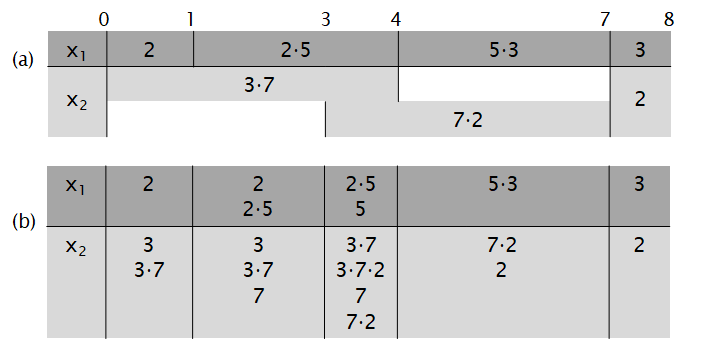
\includegraphics[scale=0.4]{valexpr.png}
	\caption{(a) Uncertainty regions and their value expressions before the segmentation. (b) The canonical segmentation of the signal and the corresponding value expressions.\label{fig:valexpr}}
\end{figure}

\subsubsection{Approximate Evaluation of Satisfaction Signals}

Let $\tau_S : [0,d) \to G_S$ be a function that maps each clock value to the interval in the canonical segmentation that it belongs to, i.e., $\tau_S(t) = [t',t'')$ where $t' \leq t < t''$ and $[t',t'') \in G_S$.
We say that two intervals $I, J \subseteq [0,d)$ with the end points $a_i < b_i$ and $a_j < b_j$ are of the \emph{same type} iff the following holds: $(a_i \in I \iff a_j \in~J) \land (b_i \in I \iff b_j \in J)$.
%For $t_1, t_2 \in [0,d)$, if $\tau_S(t_1) \neq \tau_S(t_2)$, let $(J_i)_{1 \leq i \leq k}$ the (potentially empty) sequence of intervals that are strictly between $\tau_S(t_1)$ and $\tau_S(t_2)$.

Let $(S, {\hb})$ be a distributed signal of $n$ signals, $t \in [0,d)$ be a time value such that $\tau_S(t) = [t', t'')$.
Let $I \subseteq \R_{\geq 0}$ be a time interval with the end points $a < b$.
Note that timed until can be expressed using timed eventually, timed always, and untimed until operators~\cite{MalerN13}.
We provide the semantics of our logic following this observation.

\scriptsize
\begin{align*}
	[S,t \models p] &=  f_p(\gamma(\tau_S(t), 1), \ldots, \gamma(\tau_S(t), n)) > 0 \\
	[S,t \models \lnot \varphi] &= \lnot [S,t \models \varphi] \\
	[S,t \models \varphi_1 \land \varphi_2] &= [S,t \models \varphi_1] \sqcap [S,t \models \varphi_2] \\
	[S,t \models \varphi_1 \until \varphi_2] &= \destutter(\{ [S,t \models \varphi_1] \until^b [S,t \models \varphi_2] \st \text{ if $t'' < d$ then $b \in \first([S,t'' \models \varphi_1 \until \varphi_2])$ else $b = 0$} \}) \\
	[S,t \models \LTLf_I \varphi] &= \destutter(\{ \mathsf{E}(\textit{Pr}_1) \cdot \ldots \cdot \mathsf{E}(\textit{Pr}_M) \}) \text{ where $\textit{Pr}_i \in \mathsf{profilesBetween}(I, S, \varphi, [t',t''))$ for all $1 \leq i \leq M$} \\
	[S,t \models \LTLg_I \varphi] &= \destutter(\{ \mathsf{A}(\textit{Pr}_1) \cdot \ldots \cdot \mathsf{A}(\textit{Pr}_M) \}) \text{ where $\textit{Pr}_i \in \mathsf{profilesBetween}(I, S, \varphi, [t',t''))$ for all $1 \leq i \leq M$}
\end{align*}
\normalsize

The \emph{profile} of an interval $I$ with respect to $S$ and $\varphi$ captures the value expressions for the satisfaction of $\varphi$ in $I$.
Then, $\mathsf{profilesBetween}(I, S, \varphi, J)$ is the set of profiles, with respect to $S$ and $\varphi$, of intervals of the same length and type as $I$ that coincide with the segments in $I \oplus J$.
Intuitively, we aim to compute how the satisfaction signal of $\varphi$ behaves in $I$ while we slide $I$ over $I \oplus J$.
Observe that, although there are infinitely many such windows due to denseness of time, there are only finitely many ways these windows can ``relate'' with the segments in $I \oplus J$, resulting in finitely many profiles for them.
We formalize and demonstrate this below.

Let $I \subseteq [0,d)$ be an interval with the end points $a < b$.
Given $t \in [0,d)$, we let $\mathsf{end}(t, S)$ be true iff $t=d$ or $\tau_S(t) = [t, t')$ for some $t' > t$.
Let $Q$ be the number of intervals in $G_S$ whose endpoints are strictly between $a$ and $b$.
Let $(H_k)_{1 \leq k \leq Q}$ be a (possibly empty) sequence of intervals of the canonical segmentation whose endpoints are strictly between $a$ and $b$, i.e., $H_k = [d_k, d_{k+1}) \in G_S$ and $a < d_k < d_{k+1} < b$ for all $1 \leq i \leq Q$.
We denote by $\kappa(S, a, b)$ the concatenation of the value expressions of $\varphi$ for the intervals in this sequence, i.e., $\kappa(S, a, b) = [S, s_1 \models \varphi] \cdot \ldots \cdot [S, s_Q \models \varphi]$.
We define the \emph{profile} of $I \subseteq [0,d)$ with the end points $a < b$ with respect to $S$ and $\varphi$ as follows.

\scriptsize
	\begin{equation*} 
		\mathsf{profile}(I, S, \varphi) =
		\begin{cases}
			%		[S, a \models \varphi] &\text{if $\tau_S(a) = \tau_S(b) \land \mathsf{start}(a, S) \land \mathsf{end}(b, S)$} \\
			\pfx([S, a \models \varphi]) &\text{if $\tau_S(a) = \tau_S(b) \land \mathsf{end}(a, S)$} \\
			%		\sfx([S, a \models \varphi]) &\text{if $\tau_S(a) = \tau_S(b) \land \lnot\mathsf{start}(a, S) \land \mathsf{end}(b, S)$} \\
			\infx([S, a \models \varphi]) &\text{if $\tau_S(a) = \tau_S(b) \land \lnot\mathsf{end}(a, S)$} \\
			[S, a \models \varphi] \cdot \kappa(S, a, b) \cdot \first([S, b \models \varphi]) &\text{if $\tau_S(a) \neq \tau_S(b) \land \mathsf{end}(a, S) \land \mathsf{end}(b, S) \land b \in I$} \\
			[S, a \models \varphi] \cdot \kappa(S, a, b) &\text{if $\tau_S(a) \neq \tau_S(b) \land \mathsf{end}(a, S) \land \mathsf{end}(b, S) \land b \notin I$} \\
			[S, a \models \varphi] \cdot \kappa(S, a, b) \cdot \pfx([S, a \models \varphi]) &\text{if $\tau_S(a) \neq \tau_S(b) \land \mathsf{end}(a, S) \land \lnot\mathsf{end}(b, S)$} \\
			\sfx([S, a \models \varphi]) \cdot \kappa(S, a, b) \cdot \first([S, b \models \varphi]) &\text{if $\tau_S(a) \neq \tau_S(b) \land \lnot\mathsf{end}(a, S) \land \mathsf{end}(b, S) \land b \in I$} \\
			\sfx([S, a \models \varphi]) \cdot \kappa(S, a, b) &\text{if $\tau_S(a) \neq \tau_S(b) \land \lnot\mathsf{end}(a, S) \land \mathsf{end}(b, S) \land b \notin I$} \\
			\sfx([S, a \models \varphi]) \cdot \kappa(S, a, b) \cdot \pfx([S, b \models \varphi]) &\text{if $\tau_S(a) \neq \tau_S(b) \land \lnot\mathsf{end}(a, S) \land \lnot\mathsf{end}(b, S)$} 
		\end{cases}
	\end{equation*}
\normalsize

\begin{example}
	Recall the distributed signal in \cref{ex:canonseg}.
	Let $p = (x_1 > 3)$ and $q = (x_2 > 6)$ be atomic propositions as in \cref{ex:bitwiseuntil}.
		
	First, we consider the STL formula $p \until q$.
	The value expressions of the satisfaction signals of $p$ and $q$ are respectively computed by bitwise comparison of the value expressions of $x_1$ with 3 and $x_2$ with 6.
	The resulting expressions for $q$ are given in \cref{fig:profiles}.
	We compute the values of $p \until q$ starting from the last segment $[7,8)$, which gives us $0 \mathsf{U}^0 0 = 0$.
	After handling the segment $[4,7)$ and obtain $\{ 10 \mathsf{U}^0 10, 10 \mathsf{U}^0 0 \} = \{10, 0\}$, we move to the segment $[3,4)$.
	Note that $\first(\{10, 0\}) = \{1,0\}$, therefore we compute the union of $\{01, 1\} \until^0 \{01, 010, 1, 10\}$ and $\{01, 1\} \until^1 \{01, 010, 1, 10\}$ for the segment $[3,4)$, and continue similarly with $[1,3)$ and $[0,1)$.
%	Continuing this way, we obtain the expressions $\{...\}$ for $[1,3)$ and $\{...\}$ for $[0,1)$.
	
	Now, we consider the STL formula $\LTLeventualy_{[0,1.5]} q$.
	We show the evaluation of the value expressions for the segment $[1,3)$.
	Intuitively, to compute $\LTLeventualy_{[0,1.5]} q$ in the segment $[1,3)$, one can consider a sliding window over the interval $[1,4.5)$ and compute how the behavior of the satisfaction signal of $q$ changes as the window slides.
		
	First, we need to compute the set $\mathsf{profilesBetween}([0,1.5], (x_1, x_2), p, [1,4.5))$.
	We show in \cref{fig:profiles} the profiles corresponding to how intervals of the same length and type as $[0,1.5]$ can intersect with the segments covering $[0,1.5] \oplus [1,3)$.
	
	Let us denote by $R_t$ the set of value expression of the segment starting at time $t$, given in \cref{fig:profiles}.
	Then, the six intervals in \cref{fig:profiles} correspond to the following profiles in order:
	\begin{enumerate}
		\item $\mathsf{Pr}_1 = \pfx(R_1)$
		\item $\mathsf{Pr}_2 = \infx(R_1)$
		\item $\mathsf{Pr}_3 = \sfx(R_1) \cdot \first(R_3)$
		\item $\mathsf{Pr}_4 = \sfx(R_1) \cdot \pfx(R_3)$
		\item $\mathsf{Pr}_5 = \sfx(R_1) \cdot R_3 \cdot \first(R_4)$
		\item $\mathsf{Pr}_6 = \sfx(R_1) \cdot R_3 \cdot \pfx(R_4)$
	\end{enumerate}
	Recall the sliding window analogy:
	One can imagine that we obtain these profiles by sliding a closed window of length $1.5$ over the segment $[1,3)$.
	Although there are infinitely many such windows, there are finitely many profiles; for example, $[1.2,2.7]$ and $[1.4,2.9]$ are equivalent for our purposes.
	This is because they are both strictly contained in $[1,3)$, meaning that they capture the events of $q$ that may occur strictly between the interval's endpoints.
	More specifically, they are captured by $\mathsf{Pr}_2$, as with any $t \in (1,1.5)$.
	Similarly, the profiles $\mathsf{Pr}_1$ and $\mathsf{Pr}_3$ capture respectively $t = 1$ and $t = 1.5$; the profile $\mathsf{Pr}_4$ captures $t \in (1.5,2.5)$; the profile $\mathsf{Pr}_5$ captures $t = 2.5$; and the profile $\mathsf{Pr}_6$ captures $t \in (2.5,3)$.   
	
	Applying the bitwise-eventually operator $\mathsf{E}$ to each profile, concatenating the resulting sets, and finally destuttering gives us the set of value expressions for $\LTLeventualy_{[0,1.5]} q$ in the segment $[1,3)$.
	For example, the value expression $0 10 10 10 10$ is in this set because the first two profiles each contain $0$ and the last four profiles each contain an expression equivalent to $10$ after destuttering.
	
	We remark that this example also shows how our method overapproximates the set of possible behaviors by neglecting the bookkeeping of edges.
	For example, in reality, if $x_2$ has its rising edge in $[1,3)$, then it cannot have its falling edge in $[3,4)$ due to bounded variability constant $\delta = 3$.
\end{example}

\begin{figure}
	\centering
	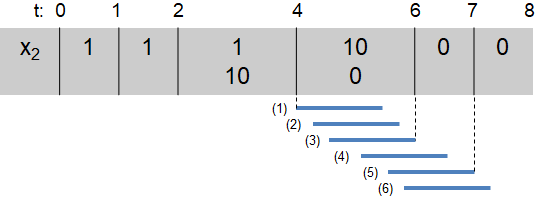
\includegraphics[scale=0.5]{profiles.png}
	\caption{The intervals representing the profiles needed to compute $\LTLeventualy_{[0,1.5]} q$ in $[1,3)$. The six black lines at the bottom show how the interval $[0,1.5]$ ``slides'' over $[1,3)$. \label{fig:profiles}}
\end{figure}